% soctepmlate unofficial - SOČ = Středoškolská odborná činnost - Czech competition
% Author: Vojtěch Boček
% Edit by: Jaroslav Páral
% Version: 2018-02-12
% Source code: https://github.com/RoboticsBrno/soctemplate/
% Base on: http://www.jcmm.cz/cz/sablona-soc.html
% License: CC BY 4.0

\documentclass{template/socthesis}

\usepackage{subcaption}
\usepackage{amsmath}
\usepackage{enumitem}
\usepackage{hyperref}
\usepackage[czech]{babel}
\usepackage{wrapfig}
\usepackage{pdfpages}


%\usepackage[
%backend=bibtex,  %if we want unicode and many other features (biber is already by default)
%style=iso-numeric, % or another iso-<style>
%sorting=nty
%]{biblatex}

%\addbibresource{text.bib}
%\addbibresource{literatura.bib}


\titlecz{Řízení robota Oscar95}
\titleen{Educational robotic arm Oscar95}
\author{Denis Kučera}
\field{12}
\school{SPŠ a VOŠ Sokolská, Brno}
\mentor{Mgr. Miroslav Burda}
\mentorstatement{Mgr. Miroslava Burdy}

% Změňte, pokud se liší
%\region{Jihomoravský}
%\placefooter{Brno 2017}

\begin{document}
	
	\maketitle
	
	\makecopyrightstatement{V~Brně}
	
	\makethanks{Děkuji svému školiteli Mgr. Miroslavovi Burdovi a dále Tomášovi Rohlínkovi, Šimonovi Skládanému a Martinovi Novákovi za obětavou pomoc, podnětné připomínky a nekonečnou trpělivost, kterou mi během práce poskytovali.}
	
	\pagestyle{empty}
	
	\section*{Anotace}
	Cílem této práce je obnovit dlouho nepoužívané robotické rameno za použití moderních technologií a udělat z něj zařízení na výuku robotiky pro studenty technických oborů.
	
	\subsection*{Klíčová slova}
	robotické rameno; Oscar95; robotika; G-code; výuka robotiky; laboratorní práce
	
	\vspace{10mm}
	
	\section*{Annotation}
	The goal of this work is restoration of old educational robotic arm, which were used in early 2000's, with help of modern technologies and make fully functional learning tool for technical subjects on high schools.
	
	\subsection*{Keywords}
	Oscar95, robotics, G-code, laboratory work, robotic arm, educational robotics
	
	\newpage
	\pagestyle{plain}
	
    \tableofcontents % vysází obsah
	
	%%% Začátek práce
	\setcounter{figure}{0}
	\setcounter{table}{0}
	\newpage
	
	%%% Úvod
	\chapter*{Úvod}
\addcontentsline{toc}{chapter}{Úvod} % přidá položku úvod do obsahu
Robotické rameno Oscar95 se v předchozích letech používalo pro výuku robotiky a automatizace. \cite{Oscar95} Během posledních několika let se toho v tomto odvětví hodně změnilo. Standardy, které vyhovovaly kdysi, jsou už nyní zastaralé. Jediné, co z původního robotického ramene vyhovuje i dnešním nárokům, je samotná konstrukce s krokovými motory. Mým cílem je proto dokončit rekonstrukci hardwaru a vytvořit software pro novou řídící desku. Dále vymyslet nové laboratorní úlohy pro studenty a udělat z Oscara95 zařízení splňující všechny technické náležitosti moderní výukové pomůcky robotiky.
\newpage
	
	%%%
	\chapter{Oscar95}

Oscar95 je školní výukové robotické rameno od firmy Elcom Education s.r.o. řízené čtyřmi krokovými motory. Rameno bylo zkonstruováno v roce 1995. Původně sloužilo jako pomůcka pro výuku automatizace a robotiky. Dalo se řídit buď ručně pomocí speciálního ovladače s tlačítky a nebo za pomocí programu v počítači. Program v počítači umožňoval studentům si vyzkoušet jednoduché řízení robota pomocí programu. Program mohli studenti psát v jazyce PASCAL, C++, BASIC, nebo také Baltazar. Poslední laboratorní práce s ním byla provedena v roce 2009 -- viz. \ref{fig:oscar_old}  na straně 
\pageref{fig:oscar_old}. Od té doby čeká na modernizaci. V některých aspektech je vzhledem ke stáří poměrně neaktuální.
Například deska s řídící elektronikou využívající ke komunikaci ještě starý canon 25 konektor. Krokové motory jsou řízené pomocí LM298 driveru, který je řízen ještě TTL logickými hodnotami. Napájení desky bylo realizováno pomocí externího 12\,V zdroje stejnosměrného napětí. Rameno umožňuje pohyb 360° kolem základny, svírání předních čelistí a pohyb svých dvou kloubů. Pohyb v kloubech a svírání přední čelisti je realizován pomocí závitových tyčí. Rameno je vyrobené převážně z hliníku, až na pár ocelových dílů a mosazné závitové tyče, aby byla celá konstrukce, pokud možno co nejlehčí. Kontrukce na první pohled působí robustně a odolně. Rameno dokáže uzvednout předmět o hmotnosti až 100 g. Rameno je vybaveno mechanickými dorazy, ale zároveň disponuje i optickými senzory koncových dojezdů. Původní deska byla vzhledem ke stáří a nekompatibilitě s dnešní pokročilou technikou nahrazena modernější. \cite{Oscar95} \cite{staveb-robot} \cite{Laborka-2009}

		


	
	%%% 
	\chapter{Hardwarové úpravy}

\section{Úpravy desky}Už od začátku práce na projektu Oscar95 bylo jasné, že původní desku plošného spoje z roku 1995 bude nutné nahradit. O to se postaral můj před\-chůd\-ce Ondřej Kratochvíl ve své maturitní práci. Nyní je k dispozici univerzální deska, se kterou můžu pracovat, popřípadě ji dále vyvíjet. \cite{Universalstepperboard} V následující kapitole se budu věnovat svým úpravám desky, které bylo nutné dodělat. Jednou z nejdůležitějších elektrotechnických úprav je bezpochyby nové napájení desky. Původně musela být nová deska napájena 12\,V zdrojem a zároveň USB kabelem 5\,V z počítače. 12\,V bylo hlavní silové napájení pro drivery krokových motorů a 5\,V pro mikrokontrolér. Přidal jsem proto stabilizátor napětí, který snižuje napětí z 12\,V na 5\,V. Připojil jsem mezi stabilizátor a hlavní napájení ze zdroje diodu. Dioda je tam proto, aby v režimu napájení z USB nedocházelo únikům do desky. Teď může deska fungovat i bez připojeného USB kabelu. Důležitou maličkostí se stalo přidání kondenzátoru k bootovacímu vývodu mikrokontroléru. Nebylo už nadále zapotřebí mačkat při každém nahrávání nového kódu mačkat bootovací tlačítko. Dalším důležitým prvkem byla detekce připojení hlavního napájení 12\,V. To jsem realizoval pomocí optočlenu připojeném na řídící vývod mikrokontroléru. Mikrokontrolér tak dostavá informaci pokaždé když dojde k připojení, nebo odpojení hlavního napájení. Poslední úpravy proběhly v rámci přidávaní nových signalizačních prvků.
\enlargethispage{20mm}
Například připojení piezo měniče, LED diod a  vypínacího/zapínacího tlačítka.  

\section{Konstrukční úpravy}Bylo potřeba dát robota do pořádku i po stránce hardwarové. Seřídit celé rameno, zkontrolovat všechny mechanické prvky, popřípadě opravit menší nedostatky z výroby. Důležitým úkolem bylo vymyslet upevnění řídící desky do základny ramene. Padlo několik návrhů, jak desku umístit. Nakonec jsme zvolili umístění mezi sloupky podstavy. Návrhů samotného řešení jsem udělal několik. Mým cílem bylo desku připevnit bez mechanického zásahu do podstavy. Počítal jsem s tím, že do budoucna pro případnou novou desku bude podstava zase jiná. Zvolil jsem proto tvar, který kopíruje vnitřní obvod podstavy. Na tuto plochu jsem potom přidal distanční sloupky pro dostatečné odsazení desky. Výsledná plocha držáku byla veliká. Se spolužákem jsme proto poté ve Sliceru upravili desku tak, aby se na její výrobu spotřebovalo co nejméně materiálu, ale zároveň byla pevná. Výsledek jsem poté upevnil u krajů základny tavnou pistolí. Poslední velmi důležitou úpravou základny Oscara jsem se inspiroval u spolužáka Šimona Skládaného. Vymyslel přední panel pro konektory vyvedené z desky. Pro umístění panelu jsem zvolil díru, která v základně zůstala po demontáži původní desky s paralelním portem. Tato díra má rozměry přibližně 8,3x6,3\,mm, což je pro uchycení dostačující. Toto řešení se mi líbilo, a proto jsem jeho nápad použil a přidal své vlastní úpravy. Panel jsem navrhoval v programu Solidworks, ve kterém se mi pracuje dobře. Vyvést ven jsem chtěl hlavně konektor USB z mikrokontroléru ESP32. Pokaždé, když by bylo potřeba nahrát nový program, muselo by se odšroubovat celé víko základny, a to je velmi nepraktické. Pro svou mechanickou odolnost a velmi dobré rozměry jsem si nakonec vybral konektor USB typ B ve standardní velikosti. Následně jsem vyrobil redukci a vymodeloval pro ni místo na panelu. Dalším důležitým prvkem je vyvedené napájení desky. To jsem vyřešil pomocí přidání napájecího DC power Jack konektoru. Pro jeho upevnění stačilo do panelu udělat díru o správném průměru. Poslední periferie, které jsem chtěl přidat na přední panel, byly signalizační prvky, tlačítko ON/OFF a dvě LED diody.\\ Stejně jako u napájecího konektoru stačilo pouze zhotovit díry se správným průměrem. Celý model panelu jsem nechal vytisknout u kamaráda na 3D tiskárně.

\section{Další úpravy robota}Na závěr jsem se ještě rozhodl dodělat chybějící podložky, vymodelovat nové nástavce do čelistí a připojit DIAG pin do driveru TMC2209. Komponenty jsem opět modeloval v programu Solidworks. U podložek jsem se snažil, aby byly co nejvíce podobné těm původním. Nejenom z hlediska vzhledu, ale i materiálu. Materiál pro tisk jsem zvolil ABS. Následně jsem nechal díl vytisknout na školní 3D tiskárně. Stejný postup jsem zopakoval i pro nástavce do čelistí. S tím rozdílem že jsem použil jiný materiál. Nástavce jsem nechal vytisknout z pružného flex materiálu, který se následně dokáže tvarem přizpůsobit. To se bude hodit v případě, že předmět nebude mít dokonale hladký povrch. Poslední významnou úpravou bylo připojení DIAG pinu do mikrokontroléru ESP32. Bez něj by totiž nefungovala funkce Stallguard\,\footnote{popsáno v kapitole 5}. Z driveru jsem drátem vyvedl tyto piny a připojil je na GPIO piny 19, 21, 22, 23, mikrokontroléru ESP32. V programu jsem následně piny nastavil a vytvořil pro ně hardwarový interrupt. Tento interrupt čeká na pulzy přicházející z DIAG pinu. \cite{BIGTREETECH-TMC2209}


	\begin{figure}
		\begin{center}
			\includegraphics[scale=0.25]{img/nastavec.png}
			\caption{Vymodelovaný nástavec do čelistí robota (vlastní fotografie)}
			\label{fig:nastavec}
		\end{center}
		\vspace{-7mm}
	\end{figure}

	
	
	%%% 
	\chapter{Ovládání pomocí aplikace}
Součástí každého moderního zařízení je umožnění řízení z mobilního telefonu. Jak již bylo zmíněno Oscar95 byl původně řízen speciálním ovladačem. Podobný ovladač jsem měl v plánu přidat také. Bylo by ale zbytečné mít v dnešní době podobný ovladač. Zjistil jsem, že existuje aplikace RBcontroller a prostředí RBGridUI vyvinuté Robotárnou, pobočkou DDM Helceletova. Rozhodl jsem proto implementovat do projektu tyto moderní prvky. Vize byla taková, že by student mohl kompletně řídit Oscara95 z telefonu nebo PC. V reálném čase by student mohl řídit pohyb robota, kontrolovat jeho pozici a případně ukládat dané souřadnice do mezipaměti a vytvořit tím souvislou trasu pohybu pro robotické rameno. Následně by student tuto trasu mohl upravovat a přidávat do ní nové body. \cite{RBController}
\section{Představení RBGridUI}
RBCgridUI je rozhraní vyvinuté také Robotárnou, které zprostředkovává 
komunikaci mezi mobilní aplikací a mikrokontrolérem ESP32. Komunikace probíhá 
pomocí wifi, nebo bluetooth připojení. Celé prostředí funguje za použití wifi síťového protokolu a webserveru běžícího na ESP32, na který 
se uživatel s aplikací připojuje. Tento webserver pracuje na samostatném jádře procesoru. Na 
druhém jádru se provádí hlavní program. Hlavní program potom načítá vzhled a funkce 
definované uživatelem v knihovně \textit{layout.hpp}. Velkou výhodou je možnost navrhnout si rozhraní pro ovládání robota uži\-va\-tel\-sky. K tomu slouží internetová stránka, ve které si lze svůj vlastní layout snadno vytvořit 
pomocí přidávání různých funkčních prvků. Celé schéma si následně můžeme upravit sami 
pomocí přidání vlastních stylů. Následně algoritmus vygeneruje kód, který pak stačí už jen vložit 
do správné složky. Práce s tímto prostředím je velmi jednoduchá a efektivní. \cite{RBGridUI}


\begin{figure}
		\begin{center}
			\includegraphics[scale=0.5]{img/rbgridui.jpg}
			\caption{Vzhled vytvořeného prostředí aplikace (vlastní fotografie)}
			\label{fig:rbgridui}
		\end{center}
		\vspace{0mm}
\end{figure}

\section{Aplikace RBController}
Samotná mobilní aplikace RBController je rovněž dílem Robotárny. Aplikace funguje na telefonech s operačním systémem Android a na počítačích s Windows nebo Linux. Umožňuje posílat instrukce z mobilního telefonu prostřednictvím bluetooth, nebo wifi. Prostředí aplikace je jednoduché a efektivní. Připojíte se na zařízení, vyberete si uživatele s jeho zařízením a následně aplikace spáruje uživatele se zařízením. Jedinou nevýhodou je, že aplikaci si nemůžou nainstalovat uživatelé iOS operačních systémů.  \cite{RBController}


	
	%%% 
	\chapter{Kolaborativní robot}
Výukový robot by měl mít vlastnosti kolaborativního robota. Vzhledem k tomu, že dochází k přímé práci člověka s robotem, je zapotřebí brát velký ohled na bezpečnost uživatele. Studenti by při práci s výukovým robotem měli být maximálně chránění. Všechny motory by měly mít proto ochranu proti přetížení, nebo rozpoznat prudce zvýšenou zátěž. Proto jsem se rozhodl přidat následu\-jí\-cí prvky kolaborativního robota. \cite{Websy}
\section{Detekce přetížení motorů}Prvním důležitým prvkem je kontrola zátěže motorů. TMC2209 driver, který je osazen na desce v Oscarovi, umožňuje spoustu užitečných funkcí. Jednou z nich je funkce Stallguard. Ta dokáže detekovat přetížení krokového motoru pomocí sledování natočení magnetického pole v motoru. Pokud driver detekuje přetížení, vyšle z jednoho svého vývodu impulz. TMC2209 detekuje tzv. \uv{Stall} motoru. Stall je událost, kdy se magnetické pole v motoru pootočí o 90 stupňů. Stallguard lze různě nastavovat. Jedním z parametrů je například \uv{stallguard threshold}. Tímto parametrem lze nastavit citlivost Stallguardu. V praxi to znamená, při jaké zátěži začne TMC2209 posílat pulzy. Následně v mikrokontroléru probíhá sledování pulzů. Pokud přijde daný pulz do mikrokontroléru, mikrokontrolér přeruší provádění hlavního programu a zastaví dané motory na kterých došlo ke Stallu. Výhodou tohoto systému je prakticky okamžité zastavení motorů v případě přetížení. Zároveň lze stejným způsobem vyřešit i koncové dojezdy motorů. Pokud motor v robotovi dojede na konec dané osy, dojde opět ke krátkému přetížení a v ten moment driver vyšle pulz. \cite{TMC2209} \cite{BIGTREETECH-TMC2209}

\begin{figure}
		\begin{center}
			\includegraphics[scale=0.5]{img/TMC2209.jpg}
			\caption{TMC2209 driver krokových motorů \cite{BIGTREETECH-TMC2209}}
			\label{fig:TMC2209}
		\end{center}
		\vspace{0mm}
\end{figure}

\section{Inteligentní řízení proudu motorů}
Další užitečnou funkcí driveru TMC2209 je \texttt{Coolstep}. Coolstep společně se Stallguardem umožňují inteligentní řízení krokových motorů. Tato technologie dokáže přizpůsobit proud motoru na základě jeho zatížení. Standardně krokové motory jedou na maximální, nebo na předem zvolený proud.
Pokud chceme maximální výkon potřebujeme tím pádem i maximální proud. Větší proud ale při trvalém provozu způsobí větší zahřívání motorů. Zvyšuje se tím riziko požáru a zároveň se tím snižuje životnost motorů. Zahříváním také vznikají větší výkonové ztráty, z toho důvodu není toto řešení vhodné pro trvalý a efektivní provoz. Proto firma Trinamic přišla s technologií Coolstep. Stejně jako u Stallguardu se zde sleduje magnetické pole motorů. Na rozdíl od Stallguardu, Coolstep neposílá pulzy, ale přímo reguluje proudy motorů na základě nastavených parametrů. Parametry Coolstepu lze nastavit zápisem dat do registrů driveru prostřednitcvím UART komunikace s mikrokontrolérem. Data v registrech zůstanou až do dalšího resetu driverů.
\cite{TMC2209}

\section{Signalizační prvky}Poslední nedílnou součástí každého kolaborativního robota jsou signalizační prvky. Signalizace může být jak světelná, tak i zvuková. V mém případě jsem se rozhodl použít obě dvě zároveň. Signalizovat lze například zapnutí robota, zastavení na koncových dojezdech nebo přetížení motorů. Světelnou signalizaci jsem realizoval ve formě dvou LED diod vyvedených na kontrolní panel. LED diody signalizují zapnutí/vypnutí robota, stand-by režim, nebo chybu programu. Zvukovou signalizaci jsem realizoval pomocí piezo měniče. Pro různé signalizace, jsem nastavil různé frekvence tónů a délku tónu. Například při zapnutí Oscara95 dojde k zvukové signalizaci ve formě sekundového 1800Hz tónu. 
	
	%%% 
	    \chapter{Implementace G-codu}Oscar95 měl jako výuková pomůcka naučit studenty programovat jednoduché příkazy v základních programovacích jazycích. Program, který byl k tomu určen je, už velmi zastaralý a pro dnešní účely prakticky nepoužitelný. Rozhodl jsem se proto místo přímého programování programovacími jazyky řídit robota zadáváním instrukcí ve formě tzv. G-codu. 
    
    \section{Co je G-code?}
    G-code je vlastně svým způsobem také programovací jazyk. S tím rozdílem že místo počítačů se pomocí něj programují průmyslové stroje. Takovými průmyslovými stroji jsou například průmysloví roboti, CNC frézy a soustruhy nebo 3D tiskárny. Pomocí G-codu přijde stroji informace z počítače o tom, kam a jakým způsobem má provést daný pohyb.První zmínky o G-codu pochází z amerického Massachusettského technologického institutu, přibližně v padesátých letech minulého století. V průběhu několika následujících let se G-code hodně změnil. Přicházely stále nové technologie. Ve výrobě se začalo přecházet na průmysl třetí generace, kdy nedílnou součástí každého výrobního procesu byl i počítač. Finální standardizovaná podoba G-codu vyšla až o třicet let později. Postupně ho začaly implementovat firmy Siemens, Sinumerik, FANUC atd. Postupně se tak G-code začal stávat nedílnou součástí nově vznikajícího průmyslového odvětví. V součastnosti většina prů\-myslových strojů pracuje právě s G-codem. O tom jsem se mohl osobně přesvědčit i na mezinárodním strojírenském veletrhu v Brně. Překvapilo mě, v jaké míře se G-code používá u 3D tiskáren. 3D tiskárny zažívají v poslední době velký nárůst popularity. Ze začátku bylo jejich použití omezené a vyráběly se pouze pro větší firmy nebo výzkumná centra. Dnes už může mít 3D tiskárnu doma každý.  G-code se proto  postupně začíná dostávat i k hobby nadšencům. \cite{G-code-wiki} \cite{G-code-explained}
    
    	\begin{figure}
    		\begin{center}
    			\includegraphics[scale=0.75]{img/gcode.jpg}
    			\caption{Ukázka G-codu \cite{G-code-foto}}
    			\label{fig:gcode}
    		\end{center}
    		\vspace{-2mm}
    	\end{figure}
    
    \section{Popis G-codu}
    
    Jak jsem již zmínil, G-code se používá převážně u průmyslových strojů mnoha různých typů. Každý G-code soubor začíná vždy znakem procenta. Následuje hlavička (header), kterou má každý výrobce trochu jinak a potom přichází na řadu písmeno G. Od toho vznikl název G-code. Za písmenem G se nachází dvojciferné číslo. Toto číslo může určovat: pracovní režim stroje, způsob vykonání daného příkazu, kalibraci, různé pokročilé konfigurace. Ve většině případů příkaz G určuje, jakým způsobem se má stroj přemístit na danou pozici. Následují souřadnice X,Y,Z. Ty určují polohu zařízení na základě Kartézské soustavy souřadnic. Můžeme se setkat i se speciální souřadnicí pro nástroj, např u CNC frézek může jít o hloubku zanoření nástroje do materiálu. Dále písmenem F se určuje rychlost. Nejčastěji bývá zadaná ve formě koeficientu základní rychlosti. Nejčastěji se rychlost udává v jednotkách mm/s. G-code soubor končí zase znakem procenta.
    \cite{G-code-wiki} \cite{G-kód}
    
    \section{Nahrání G-codu do robota}
    %\section{Prostředí Lorris toolbox}
    Další výzvou bylo tedy vymyslet řešení, jakým způsobem přizpůsobit G-code konkrétně Oscarovi. Následně vyřešit, jak G-code nahrát z PC do mikrokontroléru. Pro nahrání G-codu do robota jsem se rozhodl použít prostředí Lorris Toolbox. Lorris Toolbox je multifunkční nástroj určený pro komunikaci s různými mikrokontroléry, který byl realizován bývalým studentem naší školy Vojtěchem Bočkem. Pracuje na počítačích s operačnímy systémy Windows a Linux. Lorris pomáhá při vývoji, ladění a řízení elektronických zařízení všeho druhu, například mikrokontrolérů a  robotů.
    Lorris obsahuje čtyři nástroje: \textit{analyzér}, \textit{programátor}, \textit{terminál} a \textit{proxy}. My si pro nahrání G-codu do robota vystačíme s analyzérem a případně terminálem. Náhrávání probíhá pomocí komunikace přes USB sériovou linku s mikrokontrolérem. Z počítače pošleme informace ze zpracovaného textového souboru pomocí analyzéru v programu Lorris. Do Lorris jsme ještě před tím nahráli speciální script, který dokáže data z textového souboru převést na data pro mikrokontrolér. Data z mikrokontroléru si můžeme následně ověřit v terminálu. \cite{bibtex:Lorris}
    
    
    
    
	
	%%% 
	\chapter{Laboratorní práce z robotiky}

Labororní práce tvoří nedílnou a velmi důležitou součást výuky. 
Tato forma vzdělávání je velmi interaktivní a student si může všechny teoretické poznatky prakticky vyzkoušet. Zároveň zde často není jedno dané správné řešení, student zde může být velmi kreativní a přijít například s vlastním návrhem řešení úlohy.

\section{Realizace}
Samotná realizace laboratorní práce se řídí školním řádem, studenti během ní musí dodržovat laboratorní řád na dané škole a pokyny vyučujícího. Předpoklá\-dá se, že studenti byli na začátku školního roku poučeni o bezpečnosti. Laboratorní práce bude navazovat na znalosti z předem probraných tématických okruhů. 
Bude zařazena do výuky v návaznosti na probranou látku \textit{robotika} a \textit{PLC}. Navazující téma bude jednoduché programování mikrokontrolérů. Ideální provedení laboratorní práce je ve dvojicích, v případě nutnosti může s robotem pracovat i větší skupina studentů. Studenti budou potřebovat mobilní telefon s operačním systémem Android, nebo nootebook s operačním systémem Windows nebo Linux. Po předchozí domluvě lze zapůjčit pro práci notebook školní. Jednotlivé úlohy nejsou časově náročné. Celou laboratorní práci lze stihnout za jednu vyučovací hodinu. Nejvíce času zabere úloha improvizovaného svařovacího automatu. Méně zručným studentům tato úloha může trvat až 20 minut. Samotná inicializace robota je záležitost maximálně na 5 minut. To stejné platí i o simulované nehodě na pracovišti. Zadávání G-codu je co se týče časové náročnosti hodně individuální. Záleží jak rychle se dokážou studenti s G-codem seznámit. V poslední úloze se studenti seznamují s pohybem v souřadnicovém systému. Pro Oscara95 jsem zvolil Kartézskou soustavu souřadnic. Sférickou soustavu souřadnic jsem nevybral, protože se používají např. v zeměpisu jako zeměpisné souřadnice. Sférická soustava souřadnic je obecně vhodná spíše v problémech, které mají sférickou symetrii. Přesun na dané souřadnice jsem realizoval na základě systému relativního pozicování. Pokaždé když se rameno přemístí na danou pozici vynulují se uložené souřadnice. Rameno se tak neustále pohybuje relativně od zadávaných bodů. Do budoucna bych chtěl přidat i absolutní pozicování. V tomto případě máme pevně uložený jeden bod a ten se nemění. \cite{Kartezske-wiki} \cite{Sfericke-wiki}

\begin{figure}
		\begin{center}
			\includegraphics[scale=0.75]{img/predni_panel.png}
			\caption{Vzhled nového předního panelu Oscara95 (vlastní obrázek)}
			\label{fig:predni_panel}
		\end{center}
		\vspace{-2mm}
	\end{figure}

\section{Zadání práce}

Studenti si v laboratorní práci vyzkouší zkalibrovat robotické rameno. Otestují zároveň kolaborativní prvky robota. Například, jestli robot při spuštění vydal zvukovou a světelnou signalizaci. Následně si spočítají počet stupňů volnosti robotického ramena. Všechny tyto informace uvedou do protokolu, který budou poté zpracovávat. V případě že je robot úspěšně nastaven a připraven k provozu, může se přejít k další úloze. Studenti si vyzkouší simulovanou nehodu na pracovišti. V této úloze otestují funkci Stallguard driveru TMC2209, která dokáže při zvýšené zátěži motoru poslat informaci do mikrokontroléru a tím zastavit motor. Následující úloha slouží na otestování zručnosti a přesnosti studentů. Vyzkoušejí si řízení robota přes mobilní aplikaci případně notebook. Jejich cílem je na předem připravenou šablonu načrtnout fixem jednoduché "svary". Tím vytvoří improvizovaný svařovací automat. Výsledek poté zdokumentují a přidají jako přílohu do protokolu. V poslední úloze se seznámí s G-codem. Vyzkouší si přenos instrukcí z počítače do robotického ramena. V reálném čase uvidí výsledek svého vytvořeného programu. Forma G-codu bude odpovídat ve zjednosušené formě G-codu standardu (RS-274). Zadávané souřadnice přibližně odpovídají Kartézské soustavě souřadnic. Studenti zároveň pozorují pohyb robota v Kartézské soustavě souřadnic.  \cite{G-code-wiki}

\begin{figure}
		\begin{center}
			\includegraphics[scale=0.25]{img/Oscarove.jpg}
			\caption{Zprovoznění roboti (vlastní obrázek)}
			\label{fig:Oscarove}
		\end{center}
		\vspace{-2mm}
	\end{figure}

\section{Slovník odborných výrazů}

\begin{description}
   \item[mikrokontrolér] -- jednočipový počítač
   \item[driver] -- řídící jednotka 
   \item[analyzér] -- nástroj používaný k analýze dat
   \item[proxy] -- prostředník mezi klientem a cílovým počítačem
    \item[pin] -- vývod součástky
    \item[PLC] -- programovatelný logický automat
\end{description}





%\section{Zpracování protokolu}
	
	%%% Závěr
	\newpage
\chapter*{Závěr}
\addcontentsline{toc}{section}{Závěr}

Ve své práci se mi podařilo kompletně zrenovovat a modernizovat výukovou pomůcku Oscar95. Robot se může tím pádem školou nadále využívat pro výuku studentů a odpovídá i dnešním moderním standardům. Například ovládání pomocí mobilní aplikace přes WiFi připojení, nebo programování robota z PC přes USB port. Dále jsem přidal bezpečnostní prvky, aby robot splňoval i normy pro práci se studenty. Následně jsem zpracoval laboratorní práci z robotiky a automatizace pro studenty technických oborů. 

Do budoucna lze robota osadit senzory a přidat další interaktivní úlohy pro studenty. Během práce na projektu jsem se naučil programovat mikrokontroléry ESP32 a zároveň se zlepšil i v programování v jazyce C++. Posunul jsem svou znalost anglického jazyka na základě čtení cizích odborných dokumentací. Porozuměl jsem systému řízení krokových motorů. 
Na závěrem bych chtěl poděkovat Mgr. Miroslavovi Burdovi za věcné připomínky k samotnému textu práce.

    \newpage
	\addcontentsline{toc}{section}{Literatura a další zdroje}  
	
	\renewcommand{\refname}{Literatura a další zdroje}
	%\printbibliography[type=book,title={Books only}]
	%[type=book]
	
	\bibliographystyle{czplain}
	%\bibliographystyle{unsrtcz} % viz text Přehled LaTeXu unsrt
	\bibliography{literatura}
	
	\newpage % někdy je potřeba, aby správně vyšlo číslování stránky se seznamem obrázků v obsahu 
	
	\addcontentsline{toc}{section}{Seznam obrázků} % přidá seznam obrázků do obsahu 
	
	\listoffigures   % seznam obrázků  
	
	%%%%%%%%%%%%%%%%%%%%%%%%%%%%%%%%%%%%%%%%%%%%%%%%%%%%%%%%%%%%%%%%%%%%%%%%%%%
        \pagestyle{empty}
	\newpage
 
   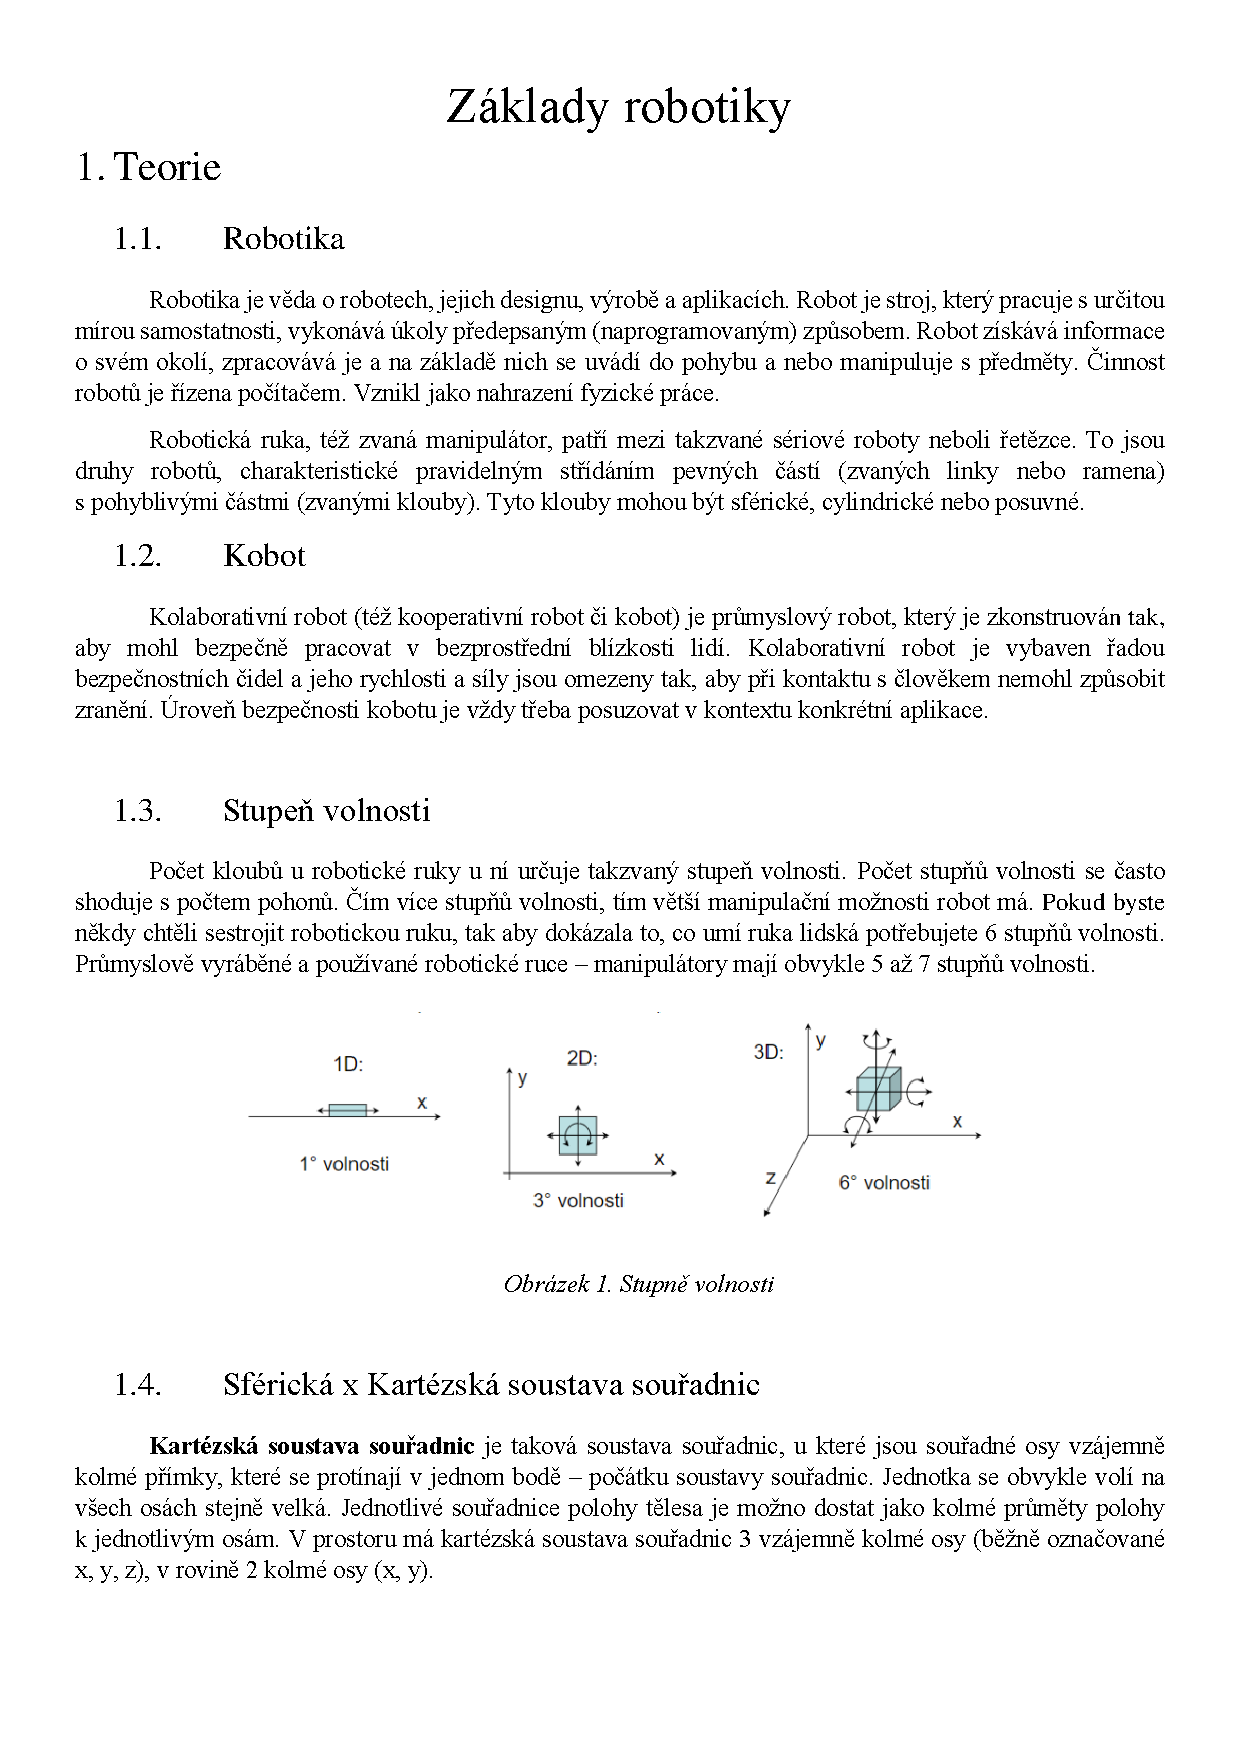
\includepdf[pagecommand=\thispagestyle{empty} \addcontentsline{toc}{section}{Laboratorní práce}, pages=1]{1 strana.pdf}
   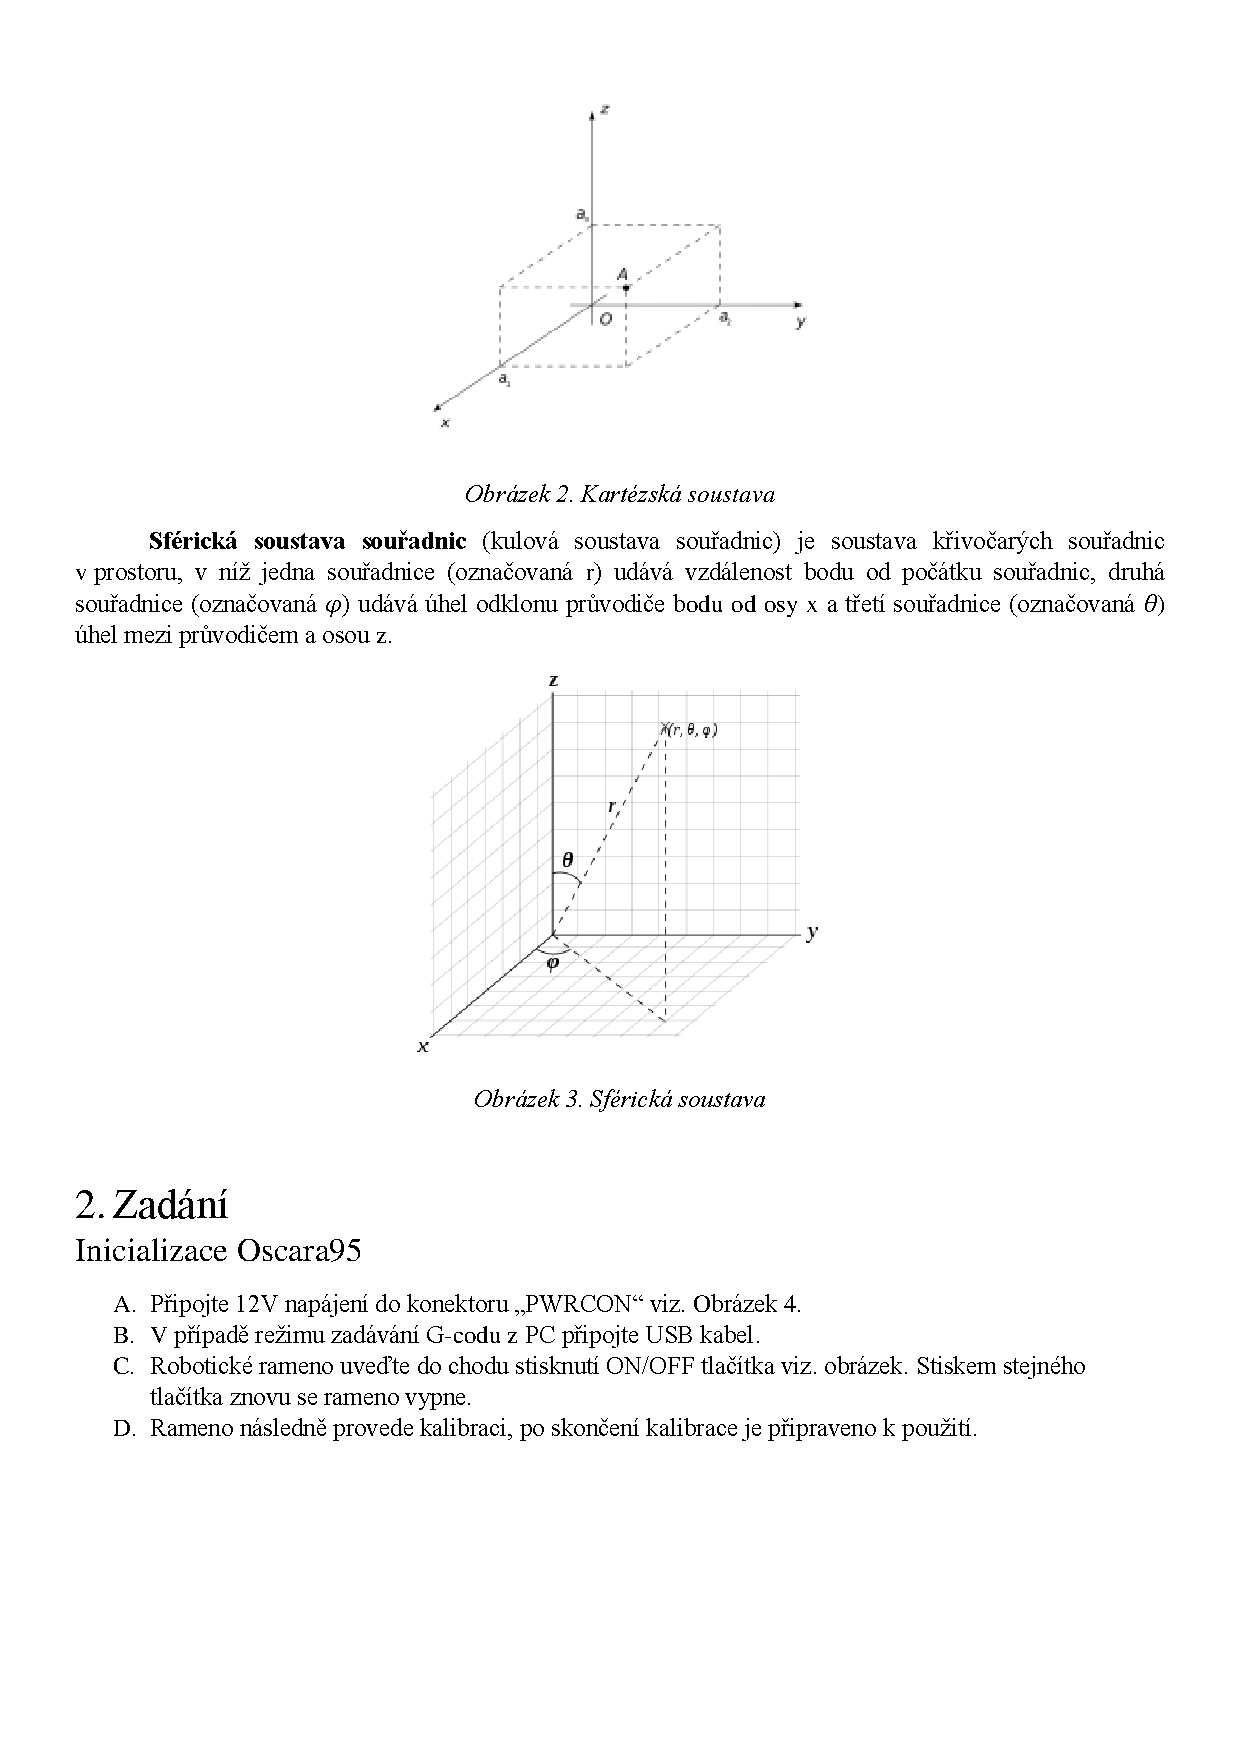
\includepdf[pagecommand=\thispagestyle{empty},pages=1-4]{4 strany.pdf}
 
	
    \section*{Další přílohy}
\enlargethispage{40mm}
    %\vspace{-50mm}
        \begin{wrapfigure}{c}{\textwidth}
		\begin{center}
			\includegraphics[scale=0.75]{img/oscar_old.jpg}
			\caption{Poslední laboratorní práce s Oscarem95 \cite{Laborka-2009}}
			\label{fig:oscar_old}
		\end{center}
		\vspace{-2mm}
	\end{wrapfigure}
	
	\addcontentsline{toc}{section}{Další přílohy} % přidá tuto položku do obsahu
	% zde budou další přílohy 
	
	%Například grafy, schémata a nebo  obrázky na celou stránku. 
	
	%\newpage
	%\addcontentsline{toc}{section}{Literatura a další zdroje}  

    
 
	%\renewcommand{\refname}{Literatura a další zdroje}
	%\printbibliography[type=book,title={Books only}]
	%[type=book]
	
	%\bibliographystyle{czplain}
	%\bibliographystyle{unsrtcz} % viz text Přehled LaTeXu unsrt
	%\bibliography{literatura}
    % \printbibliography[title={Seznam literatury, pramenů a internetových zdrojů}]    
	
	%\listoffigures
	%\addcontentsline{toc}{section}{Seznam obrázků}
	
	%\listoftables
	%\addcontentsline{toc}{section}{Seznam tabulek}
	
	%\listoflistedequation
	%\addcontentsline{toc}{section}{Seznam rovnic}
	
\end{document}
